  
\documentclass{beamer}
\usepackage{listings}
\usepackage{graphicx}
\usepackage{epstopdf}
\usepackage{hyperref}

\lstset{
		tabsize=4,
        basicstyle=\scriptsize,
        %upquote=true,
        aboveskip={1.5\baselineskip},
        columns=fixed,
        showstringspaces=false,
        extendedchars=true,
        breaklines=true,
        prebreak = \raisebox{0ex}[0ex][0ex]{\ensuremath{\hookleftarrow}},
		frame=tRBl,
		%frameround=tttf,
		numbers=left,
		numberstyle=\tiny,
		numbersep=5pt,
        showtabs=false,
        showspaces=false,
        showstringspaces=false,
        identifierstyle=\ttfamily,
        keywordstyle=\color[rgb]{0,0,1},
        commentstyle=\color[rgb]{0.133,0.545,0.133},
        stringstyle=\color[rgb]{0.627,0.126,0.941},
        aboveskip=5pt
}

\usetheme{AnnArbor}
\usecolortheme{beaver}
\setbeamertemplate{note page}[plain]
\begin{document}

\title{Introduction to Testing}
%\subtitle{example using Sinatra}
\author[Konstantinos Karasavvas]{Konstantinos Karasavvas} %\\{\small Software Architect and Engineer}}

%http://www.linkedin.com/pub/konstantinos-karasavvas/14/64b/14b
\institute{CITY College}
\date{\today} 

\begin{frame}
  \titlepage
\end{frame}

\begin{frame}
\setcounter{tocdepth}{1}
\frametitle{Table of contents}
\tableofcontents
\end{frame} 





\section{Testing Software} 
\subsection{Testing Methods}
\begin{frame}[fragile]\frametitle{Testing Methods} 
  \begin{itemize}
    \item Static testing
    \begin{itemize}
      \item reviews or walkthroughs
    \end{itemize}

    \item Dynamic testing
    \begin{itemize}
      \item automatic code testing
    \end{itemize}
    
    \item White box testing
    \begin{itemize}
      \item internal workings of software code
    \end{itemize}
        
    \item Black box testing
    \begin{itemize}
      \item functionality of software code
    \end{itemize}
  \end{itemize}
\end{frame}


\subsection{Testing Levels}
\begin{frame}[fragile]\frametitle{Testing Levels} 
  \begin{itemize}
    \item Unit testing
    \begin{itemize}
      \item test individual units of code (and composed units)
      \item procedural: typically functions
      \item Object-oriented: typically classes
      \item white box testing
    \end{itemize}

    \item Integration testing
    \begin{itemize}
      \item tests subsystem communications through their interfaces
      \item black box testing from the subsystem's perspective
      \item white box testing from the system's perspective
      \item can used to verify functional, performance, and reliability requirements
    \end{itemize}
    
    \item System testing
    \begin{itemize}
      \item tests complete system
      \item black box testing
      \item can used to verify functional, performance, and reliability requirements
    \end{itemize}
  \end{itemize}
\end{frame}



%http://soundsoftware.ac.uk/unit-testing-why-bother
%http://stackoverflow.com/questions/67299/is-unit-testing-worth-the-effort

\section{Why Testing?}
\begin{frame}[fragile]\frametitle{Why Testing?} 
  \begin{itemize}
    \item Better code quality
    \begin{itemize}
      \item the code could have bugs
      \item the tests could have bugs
      \item but chances for both to have bugs is low
    \end{itemize}

    \item Increased confidence
    \begin{itemize}
      \item via regression testing
      \item Tests ensure that everything is tested every time
    \end{itemize}

    \item Allows quicker/bigger changes to code
    \begin{itemize}
      \item If the old tests work then no need to check if something broke
      \item depends on testing coverage
    \end{itemize}
    
    \item Good unit tests help you define and document the intended functionality better
    
  \end{itemize}
\end{frame}


\section{Unit Testing} 
\begin{frame}[fragile]\frametitle{Unit Testing, Example} 
  \begin{lstlisting}[language=ruby, escapechar={^}]
# File:  simple_number.rb
 
class SimpleNumber
 
  def initialize(num)
    raise unless num.is_a?(Numeric)
    @x = num
  end
 
  def add(y)
    @x + y
  end
 
  def multiply(y)
    @x * y
  end
 
end
  \end{lstlisting}
\end{frame}



\begin{frame}[fragile]\frametitle{Unit Testing, Example, cont.} 
  \begin{lstlisting}[language=ruby, escapechar={^}]
# File:  tc_simple_number.rb
 
require_relative "simple_number"
require "test/unit"
 
class TestSimpleNumber < Test::Unit::TestCase
 
  def test_simple
    assert_equal(4, SimpleNumber.new(2).add(2) )
    assert_equal(6, SimpleNumber.new(2).multiply(3) )
  end
 
end
  \end{lstlisting}
\end{frame}



\begin{frame}[fragile]\frametitle{Unit Testing, Example, cont.} 
  \begin{lstlisting}[language=bash, escapechar={^}]
$ ruby tc_simple_number.rb
Loaded suite tc_simple_number
Started
.
Finished in 0.002695 seconds.

1 tests, 2 assertions, 0 failures, 0 errors
  \end{lstlisting}
\end{frame}



\begin{frame}[fragile]\frametitle{Unit Testing, Example, cont.} 
  \begin{lstlisting}[language=ruby, escapechar={^}]
# File:  tc_simple_number2.rb
 
require_relative "simple_number"
require "test/unit"
 
class TestSimpleNumber < Test::Unit::TestCase
 
  def test_simple
    assert_equal(4, SimpleNumber.new(2).add(2) )
    assert_equal(4, SimpleNumber.new(2).multiply(2) )
  end
 
  def test_typecheck
    assert_raise( RuntimeError ) { SimpleNumber.new('a') }
  end
 
  def test_failure
    assert_equal(3, SimpleNumber.new(2).add(2), "Adding doesn't work" )
  end
 
end
  \end{lstlisting}
\end{frame}



\begin{frame}[fragile]\frametitle{Unit Testing, Example, cont.} 
  \begin{lstlisting}[language=bash, escapechar={^}]
$ ruby tc_simple_number2.rb
Loaded suite tc_simple_number2
Started
...
Finished in 0.038617 seconds.
 
  1) Failure:
test_failure(TestSimpleNumber) [tc_simple_number2.rb:16]:
Adding doesn't work.
<3> expected but was
<4>.
 
3 tests, 4 assertions, 1 failures, 0 errors
  \end{lstlisting}
\end{frame}



\begin{frame}[fragile]\frametitle{Unit Testing, Example, cont.} 
  \begin{lstlisting}[language=ruby, escapechar={^}]
# File:  tc_simple_number3.rb
 
require "./simple_number"
require "test/unit"
 
class TestSimpleNumber < Test::Unit::TestCase
 
  def setup
    @num = SimpleNumber.new(2)
  end
 
  def teardown
  end
 
  def test_simple
    assert_equal(4, @num.add(2) )
  end
 
  def test_simple2
    assert_equal(4, @num.multiply(2) )
  end
 
end
  \end{lstlisting}
\end{frame}



\section{TDD/BDD}
\begin{frame}[fragile]\frametitle{Test-driven development (TDD)} 
  \begin{itemize}
    \item Software development process
    \begin{itemize}
      \item first the developer writes the automated test -- will fail
      \item then he/she writes the minimum amount of code to pass the test
      \item finally he/she refactors the new code to acceptable standards
    \end{itemize}
    
    \item Forces developers to think about their code before writing it
    \item Must think of the ways his code (objects) interact with other code (objects/mock objects)
    \item Forces developers to think about interactions and interfaces before writing code
  \end{itemize}
\end{frame}



\begin{frame}[fragile]\frametitle{Mock Objects} 
  \begin{itemize}
    \item Used to \textit{simulate} object's behaviour for testing code which
    \begin{itemize}
      \item depends on an external resource (WS, filesystem, DB, mail server, ...)
      \item would involve a large amount of non-reusable setup and fixture data
      \item relies on features which are particularly computationally expensive
      \item depends on unwritten objects
    \end{itemize}
  \end{itemize}
\end{frame}




\begin{frame}[fragile]\frametitle{Specifications and BDD} 
  \begin{itemize}
    \item Human readable specifications that direct and validate code
    \begin{itemize}
      \item Unit testing at a more abstract level
      \item Tests behaviour
    \end{itemize}
    \item Behaviour Driven Development combines aspects of
    \begin{itemize}
      \item Acceptance Test Driven Planning
      \item Domain Driven Design
      \item Test Driven Development
    \end{itemize}
    
    \item Ruby's RSpec
    \begin{quote}
      Domain Specific Language for describing the expected behaviour of a system with executable examples.
    \end{quote}
    \begin{itemize}
      \item instead of assertions it uses describers
      \item ...you describe a class, method, etc.
      \item ...and then you state expectations
    \end{itemize}
  \end{itemize}
\end{frame}




\section{RSpec}
\begin{frame}[fragile]\frametitle{RSpec} 

  \begin{lstlisting}[language=ruby, escapechar={^}]
$ gem install rspec
  \end{lstlisting}
  \pause
  
  \begin{itemize}
    \item \texttt{rspec\_example}
    \begin{itemize}
      \item \texttt{spec}
      \item \texttt{lib}
    \end{itemize}
  \end{itemize}
  \pause 
   
  \begin{lstlisting}[language=ruby, escapechar={^}]
# add_spec.rb                                                                                                                                                                                                        
describe "add function" do
  it "adds two numbers" do
    add(2,3).should == 5
  end 
end
  \end{lstlisting}
  \pause
  
  \begin{lstlisting}[language=bash, escapechar={^}]
$ rspec
  \end{lstlisting}

\end{frame}



\begin{frame}[fragile]\frametitle{RSpec, cont.} 

  \begin{lstlisting}[language=bash, escapechar={^}]
Failures:

  1) add function adds two numbers
     Failure/Error: add(2,3).should == 5
     NoMethodError:
       undefined method `add' for #<RSpec::Core::ExampleGroup::Nested_1:0x0000000193fe30>
     # ./spec/add_spec.rb:5:in `block (2 levels) in <top (required)>'

Finished in 0.00077 seconds
1 example, 1 failure

  \end{lstlisting}

\end{frame}



\begin{frame}[fragile]\frametitle{RSpec, cont.} 

  \lstinputlisting[language=ruby]{code/rspec_example/lib/add.rb}
  \pause

  \lstinputlisting[language=ruby]{code/rspec_example/spec/add_spec.rb}
  \pause

  \begin{lstlisting}[language=bash, escapechar={^}]
$ rspec
.

Finished in 0.00076 seconds
1 example, 0 failures
  \end{lstlisting}

\end{frame}


\section{Rack Testing}
\begin{frame}[fragile]\frametitle{Rack Testing} 
  \begin{lstlisting}[language=ruby, escapechar={^}]
$ gem install rack-test
  \end{lstlisting}
  \pause

  \lstinputlisting[language=ruby]{code/rack_example/my_app.rb}
  \pause

  \lstinputlisting[language=ruby]{code/rack_example/config.ru}
  
\end{frame}


\begin{frame}[fragile]\frametitle{Rack Testing, cont.} 

  \lstinputlisting[language=ruby]{code/rack_example/spec/sinatra_spec.rb}
  
\end{frame}



\begin{frame}[fragile]\frametitle{Rack Testing, cont.} 

  \begin{lstlisting}[language=bash, escapechar={^}]
$ rspec 
.

Finished in 0.06143 seconds
1 example, 0 failures
  \end{lstlisting}
  
\end{frame}


\section{Selenium}
\begin{frame}[fragile]\frametitle{Functional Testing with Selenium} 

  \begin{itemize}
    \item Selenium is a set of different tools to enable test automation
    \begin{itemize}
      \item Selenium IDE
      \item Selenium Server
      \item ...
    \end{itemize}

    \item Selenium IDE
    \begin{itemize}
      \item Plugin for Firefox
      \item Captures user actions and allows assertions on them
      \begin{itemize}
        \item \texttt{assertXXX}; e.g. \texttt{assertText}
        \item \texttt{verifyXXX}; e.g. \texttt{verifyText}
      \end{itemize}
      \item verify allows test to continue, assert does not
    \end{itemize}
    
    \item Need to install Selenium IDE plugin to Firefox
  \end{itemize}
  
\end{frame}


\begin{frame}[fragile]\frametitle{Selenium IDE Example} 

  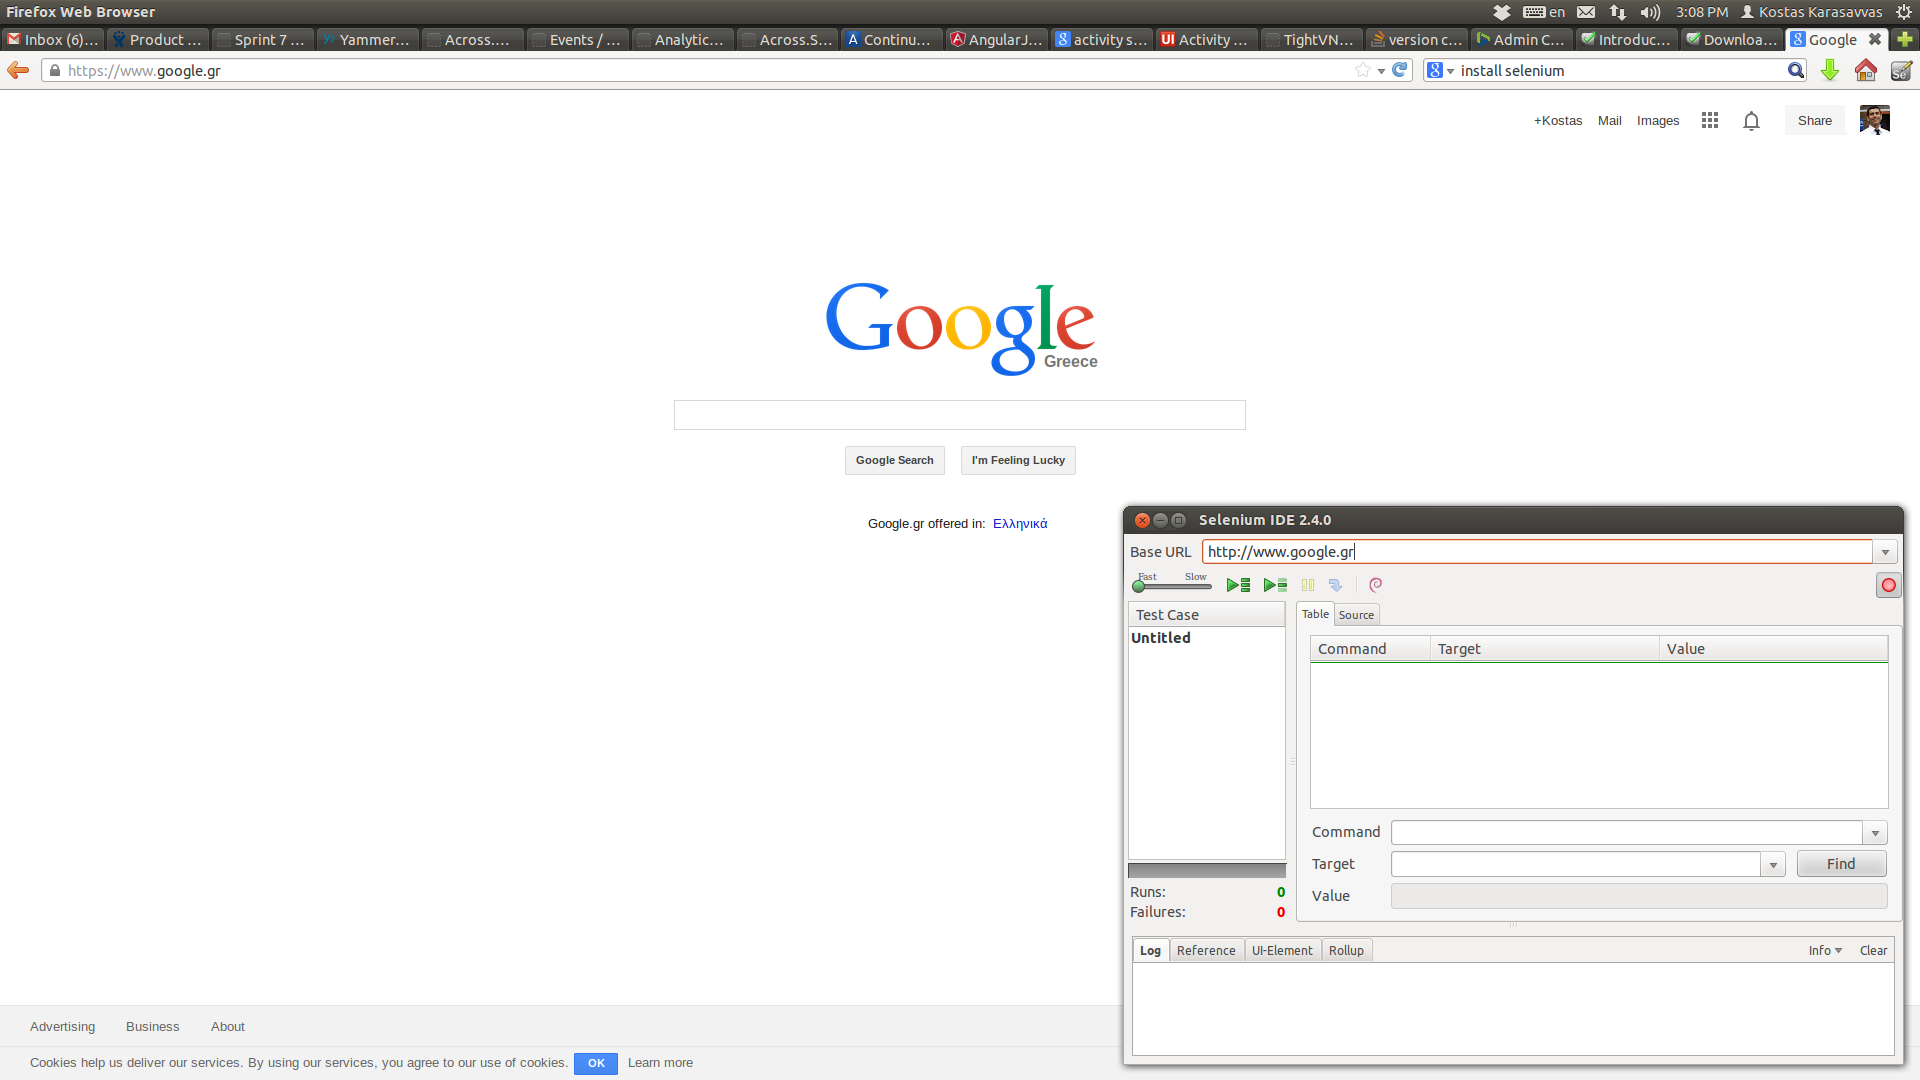
\includegraphics[scale=0.18]{images/starting_selenium_ide.png}
  
\end{frame}



\begin{frame}[fragile]\frametitle{Selenium IDE Example, cont.} 

  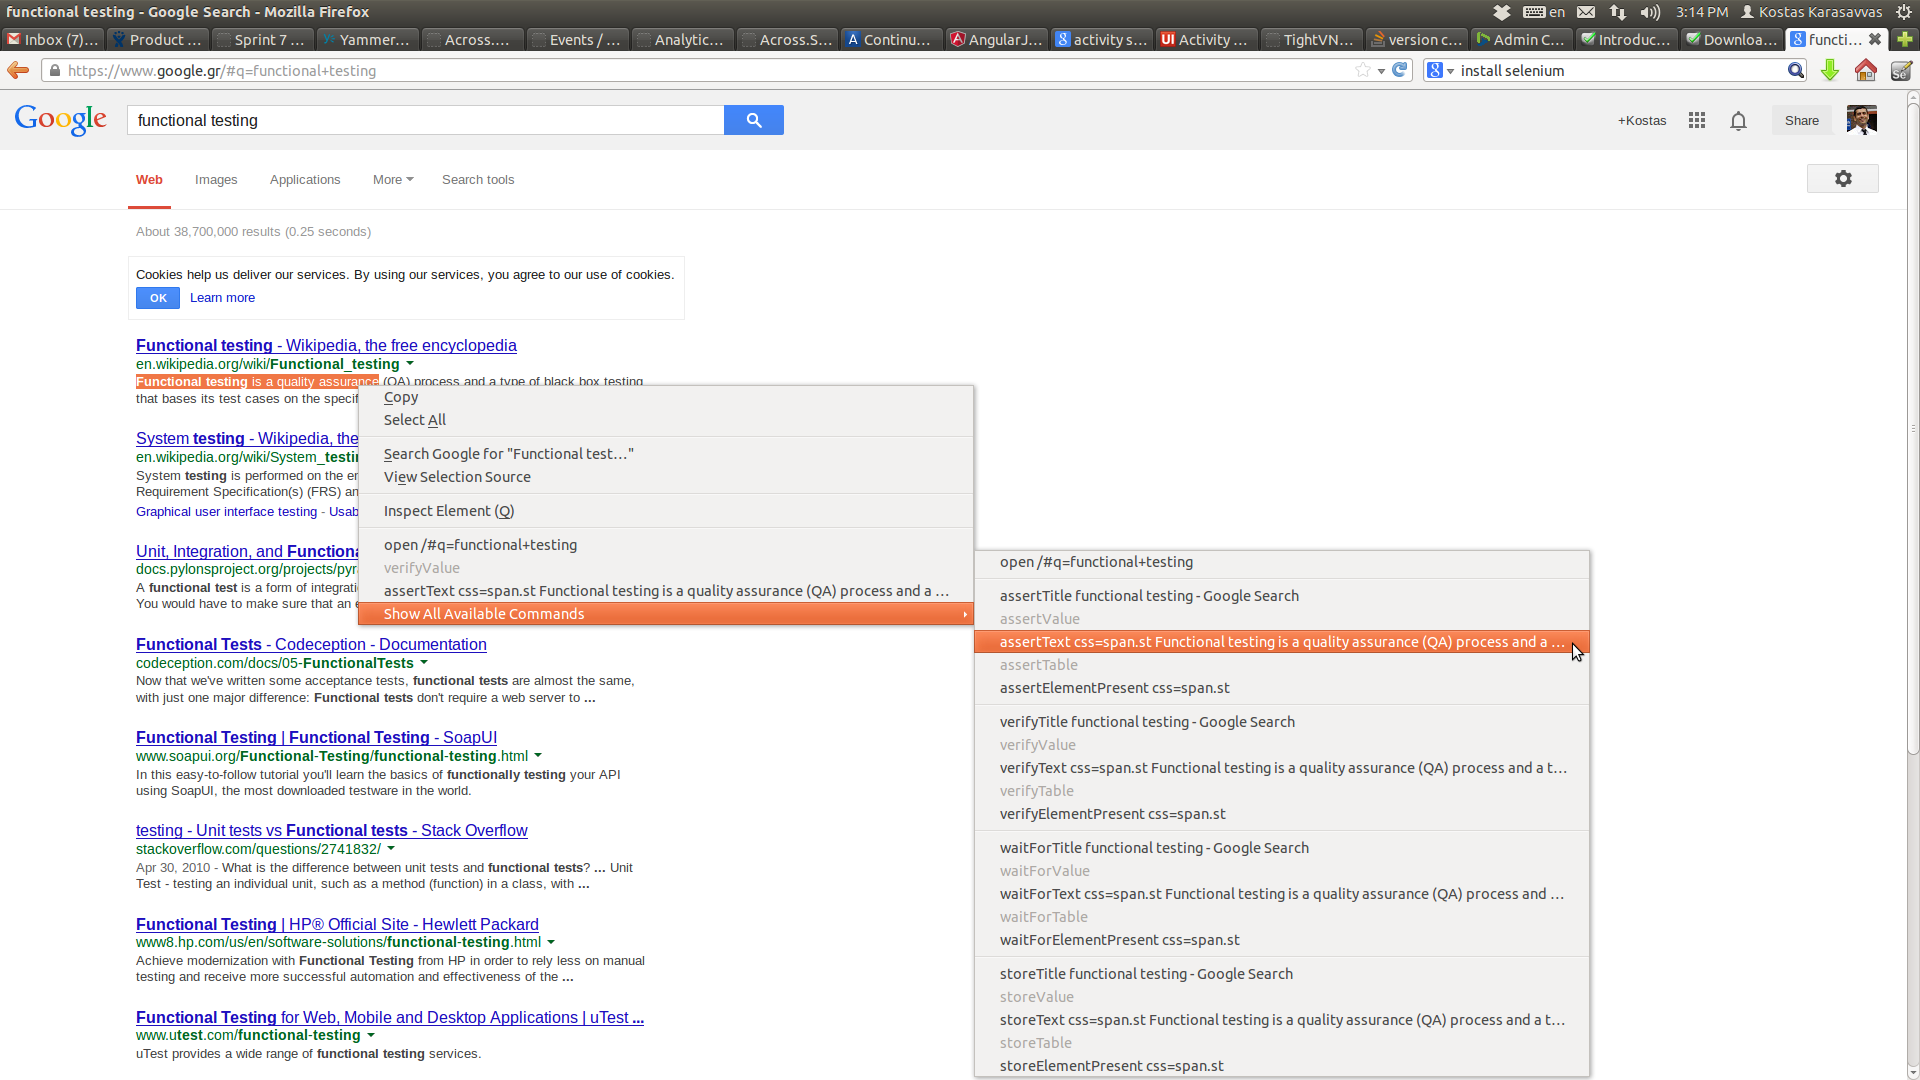
\includegraphics[scale=0.18]{images/selenium_add_assertions.png}
  
\end{frame}


\begin{frame}[fragile]\frametitle{Selenium IDE Example, cont.} 

  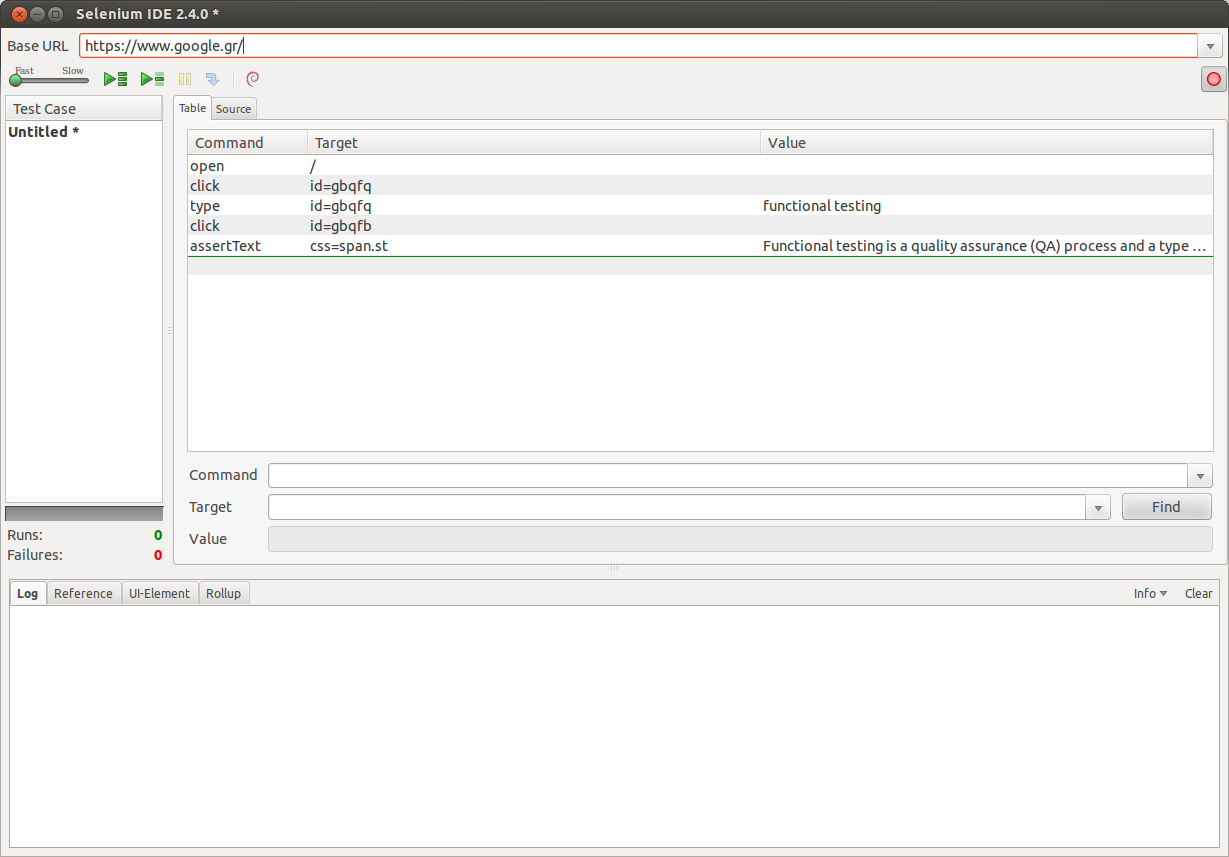
\includegraphics[scale=0.28]{images/Selenium_IDE.png}
  
\end{frame}


\begin{frame}[fragile]\frametitle{Selenium IDE Example, cont.} 

  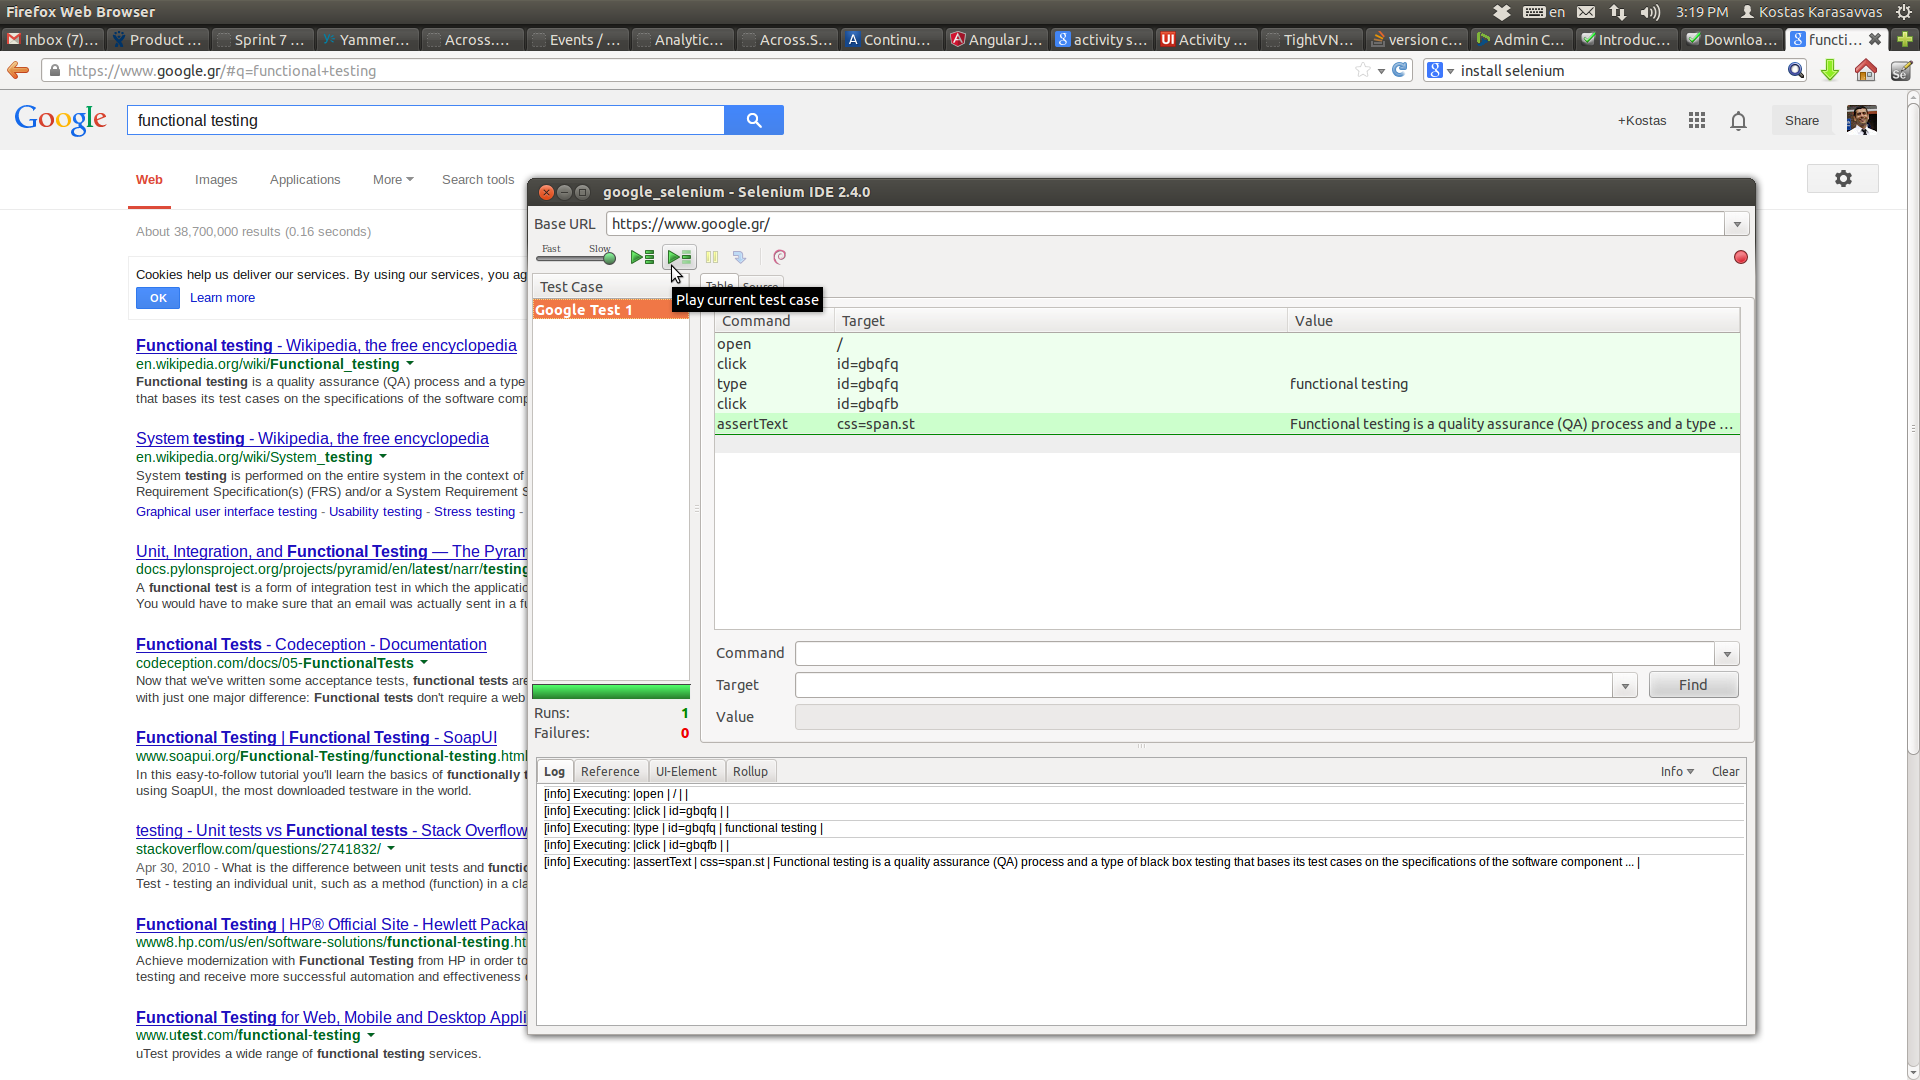
\includegraphics[scale=0.18]{images/selenium_running_test.png}
  
\end{frame}


\begin{frame}[fragile]\frametitle{Selenium IDE Example, cont.} 

  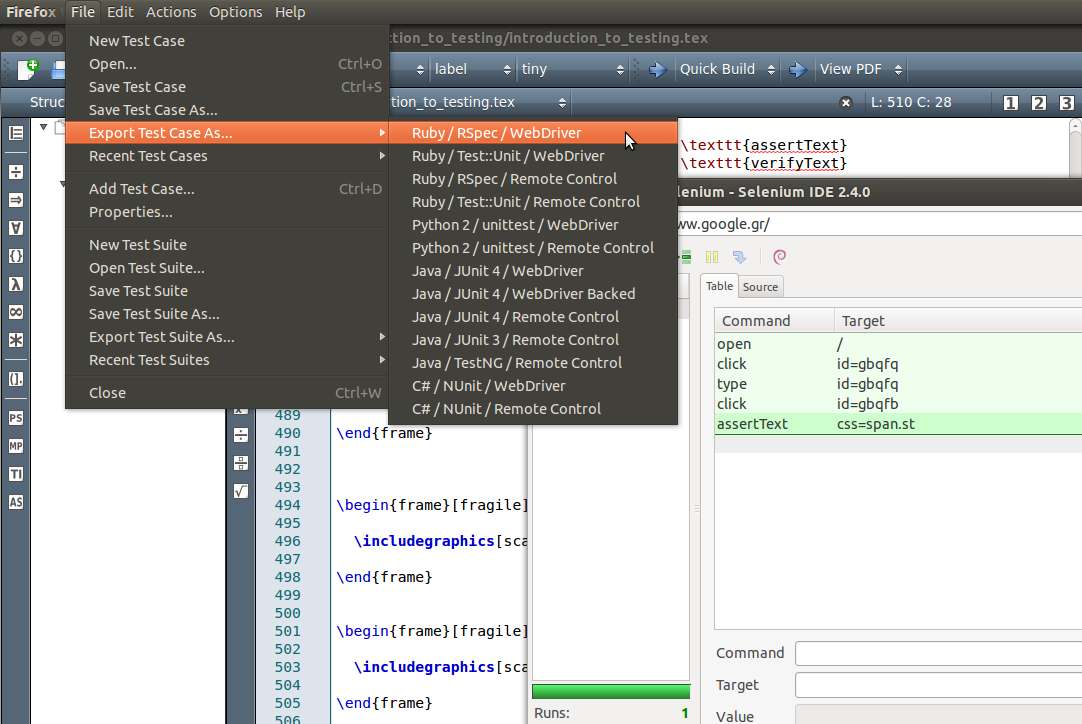
\includegraphics[scale=0.32]{images/export_to_rspec.png}
  
\end{frame}


\begin{frame}[fragile]\frametitle{Selenium and RSpecs} 

  \begin{lstlisting}[language=ruby, basicstyle=\tiny, escapechar={^}]
require "json"
require "selenium-webdriver"
require "rspec"
include RSpec::Expectations

describe "GoogleTest1" do

  before(:each) do
    @driver = Selenium::WebDriver.for :firefox
    @base_url = "https://www.google.gr/"
    @accept_next_alert = true
    @driver.manage.timeouts.implicit_wait = 30
    @verification_errors = []
  end
  
  after(:each) do
    @driver.quit
    @verification_errors.should == []
  end
  
  it "test_google_test1" do
    @driver.get(@base_url + "/")
    @driver.find_element(:id, "gbqfq").click
    @driver.find_element(:id, "gbqfq").clear
    @driver.find_element(:id, "gbqfq").send_keys "functional testing"
    @driver.find_element(:id, "gbqfb").click
    (@driver.find_element(:css, "span.st").text).should == "Functional testing is a quality assurance (QA) process and a type of black box testing that bases its test cases on the specifications of the software component ..."
  end
...
  \end{lstlisting}
  
\end{frame}


\begin{frame}[fragile]\frametitle{Selenium and RSpecs} 

  \begin{lstlisting}[language=bash, escapechar={^}]
$ gem install rspec selenium-webdriver
  \end{lstlisting}

  \begin{lstlisting}[language=bash, escapechar={^}]
$ rspec spec/google_selenium_rspec.rb
.

Finished in 16.47 seconds
1 example, 0 failures
  \end{lstlisting}
  
  \begin{itemize}
    \item default browser will open and test \textit{driven} visually
  \end{itemize}
  
\end{frame}



\end{document}
